\documentclass[10pt]{article}
\usepackage{tikz}
\usetikzlibrary{shapes.misc}
\usepackage[margin=0cm]{geometry}
\pagestyle{empty}
\tikzstyle{every node}=[cross out, draw, red]

\begin{document}

\vspace*{\fill}
\begin{center}
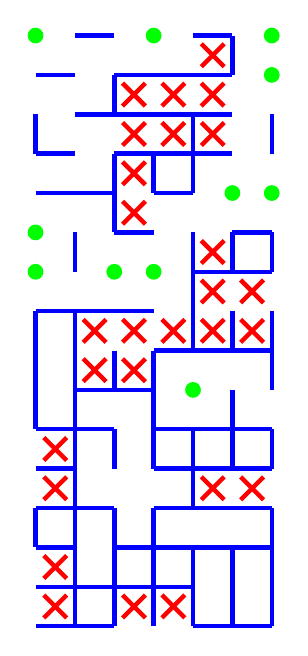
\begin{tikzpicture}[x=0.5cm, y=-0.5cm, ultra thick, blue]
% Walls
    \draw (1,0) -- (2,0);
    \draw (4,0) -- (5,0);
    \draw (0,1) -- (1,1);
    \draw (2,1) -- (5,1);
    \draw (1,2) -- (5,2);
    \draw (0,3) -- (1,3);
    \draw (2,3) -- (5,3);
    \draw (0,4) -- (2,4);
    \draw (3,4) -- (4,4);
    \draw (2,5) -- (3,5);
    \draw (5,5) -- (6,5);
    \draw (4,6) -- (6,6);
    \draw (0,7) -- (3,7);
    \draw (3,8) -- (6,8);
    \draw (1,9) -- (3,9);
    \draw (0,10) -- (2,10);
    \draw (3,10) -- (6,10);
    \draw (0,11) -- (1,11);
    \draw (3,11) -- (6,11);
    \draw (0,12) -- (2,12);
    \draw (3,12) -- (6,12);
    \draw (0,13) -- (1,13);
    \draw (2,13) -- (6,13);
    \draw (0,14) -- (4,14);
    \draw (0,15) -- (2,15);
    \draw (4,15) -- (6,15);
    \draw (0,2) -- (0,3);
    \draw (0,7) -- (0,10);
    \draw (0,12) -- (0,13);
    \draw (1,5) -- (1,6);
    \draw (1,7) -- (1,15);
    \draw (2,1) -- (2,2);
    \draw (2,3) -- (2,5);
    \draw (2,8) -- (2,9);
    \draw (2,10) -- (2,11);
    \draw (2,12) -- (2,15);
    \draw (3,3) -- (3,4);
    \draw (3,8) -- (3,11);
    \draw (3,12) -- (3,15);
    \draw (4,2) -- (4,4);
    \draw (4,5) -- (4,8);
    \draw (4,10) -- (4,12);
    \draw (4,13) -- (4,15);
    \draw (5,0) -- (5,1);
    \draw (5,5) -- (5,6);
    \draw (5,7) -- (5,8);
    \draw (5,9) -- (5,11);
    \draw (5,13) -- (5,15);
    \draw (6,2) -- (6,3);
    \draw (6,5) -- (6,6);
    \draw (6,7) -- (6,9);
    \draw (6,10) -- (6,11);
    \draw (6,12) -- (6,15);
% Pillars
    \fill[green] (0,0) circle(0.2);
    \fill[green] (3,0) circle(0.2);
    \fill[green] (6,0) circle(0.2);
    \fill[green] (6,1) circle(0.2);
    \fill[green] (5,4) circle(0.2);
    \fill[green] (6,4) circle(0.2);
    \fill[green] (0,5) circle(0.2);
    \fill[green] (0,6) circle(0.2);
    \fill[green] (2,6) circle(0.2);
    \fill[green] (3,6) circle(0.2);
    \fill[green] (4,9) circle(0.2);
% Inner points in accessible cul-de-sacs
    \node at (4.5,0.5) {};
    \node at (2.5,1.5) {};
    \node at (3.5,1.5) {};
    \node at (4.5,1.5) {};
    \node at (2.5,2.5) {};
    \node at (3.5,2.5) {};
    \node at (4.5,2.5) {};
    \node at (2.5,3.5) {};
    \node at (2.5,4.5) {};
    \node at (4.5,5.5) {};
    \node at (4.5,6.5) {};
    \node at (5.5,6.5) {};
    \node at (1.5,7.5) {};
    \node at (2.5,7.5) {};
    \node at (3.5,7.5) {};
    \node at (4.5,7.5) {};
    \node at (5.5,7.5) {};
    \node at (1.5,8.5) {};
    \node at (2.5,8.5) {};
    \node at (0.5,10.5) {};
    \node at (0.5,11.5) {};
    \node at (4.5,11.5) {};
    \node at (5.5,11.5) {};
    \node at (0.5,13.5) {};
    \node at (0.5,14.5) {};
    \node at (2.5,14.5) {};
    \node at (3.5,14.5) {};
% Entry-exit paths without intersections
\end{tikzpicture}
\end{center}
\vspace*{\fill}

\end{document}
